\documentclass{beamer}
\usepackage[spanish]{babel}
\usepackage[T1]{fontenc}
\usepackage{bookmark}
\usepackage[utf8]{inputenc}
\usepackage{graphicx}
\usepackage{listings}
\usepackage{xcolor}
\usepackage{tikz}
\usetikzlibrary{positioning,arrows,shapes}

% Tema de Beamer
\usetheme{Madrid}
\usecolortheme{default}
\setbeamertemplate{navigation symbols}{}
\setbeamertemplate{footline}[frame number]

% Configuración para que listings maneje correctamente caracteres UTF-8
\lstset{
  literate=%
  {á}{{\'a}}1
  {é}{{\'e}}1
  {í}{{\'i}}1
  {ó}{{\'o}}1
  {ú}{{\'u}}1
  {ü}{{\"u}}1
  {ñ}{{\~n}}1
  {Á}{{\'A}}1
  {É}{{\'E}}1
  {Í}{{\'I}}1
  {Ó}{{\'O}}1
  {Ú}{{\'U}}1
}

% Colores para código
\definecolor{codegreen}{rgb}{0,0.6,0}
\definecolor{codegray}{rgb}{0.5,0.5,0.5}
\definecolor{codepurple}{rgb}{0.58,0,0.82}
\definecolor{backcolour}{rgb}{0.95,0.95,0.92}

\lstdefinestyle{mystyle}{
    backgroundcolor=\color{backcolour},   
    commentstyle=\color{codegreen},
    keywordstyle=\color{codepurple},
    numberstyle=\tiny\color{codegray},
    stringstyle=\color{codegreen},
    basicstyle=\ttfamily\footnotesize,
    breakatwhitespace=false,         
    breaklines=true,                 
    captionpos=b,                    
    keepspaces=true,                 
    numbers=left,                    
    numbersep=5pt,                  
    showspaces=false,                
    showstringspaces=false,
    showtabs=false,                  
    tabsize=2
}

\lstset{style=mystyle}

\title{Implementación de XSLT en una Aplicación Web para Visualización de Estaciones de Carga EV}
\subtitle{Tópicos de Ciencias de la Computación III}
\author{ Andre Pacheco | Walter Rivera | Sergio Pezo | Gustavo Delgado | Gabriel Barrientos }
\date{\today}
\institute{Universidad Nacional de Ingeniería}

% Asegurar que se cargue hyperref
\usepackage{hyperref}
\hypersetup{colorlinks=true, linkcolor=blue}

\AtBeginSection[]
{
  \begin{frame}
  \frametitle{Contenido}
  \tableofcontents[currentsection]
  \end{frame}
}

\begin{document}

% Portada
\begin{frame}
  \titlepage
\end{frame}

% Índice
\begin{frame}{Contenido}
  \tableofcontents
\end{frame}

% INTRODUCCIÓN
\section{Introducción}

  \begin{frame}
  \frametitle{¿De qué trata esta presentación?}
  En esta presentación explicaremos cómo se desarrolló una aplicación web que muestra estaciones de carga para autos eléctricos, usando una tecnología llamada XSLT. Iremos paso a paso, desde lo más básico hasta cómo se integra todo en el proyecto.
  \end{frame}

  \begin{frame}
  \frametitle{¿Qué es XSLT?}
  \begin{itemize}
      \item XSLT (eXtensible Stylesheet Language Transformations) es un lenguaje que sirve para transformar datos en formato XML a otros formatos, como HTML.
      \item Es muy útil cuando queremos mostrar datos estructurados en una página web.
      \item Permite separar los datos de la presentación visual.
      \item En nuestra aplicación, lo usamos para convertir datos de estaciones de carga en una interfaz web completa y dinámica.
  \end{itemize}
  \end{frame}

% CONTEXTO DEL PROYECTO
\section{Contexto del Proyecto}

  \begin{frame}
  \frametitle{¿Qué problema resuelve nuestro proyecto?}
  Como problema de ejemplo el profesor del curso asignó un archivo xml que incluye
  la lista de las direcciones de estaciones de carga de vehículos eléctricos. El objetivo es crear 
  una aplicación web que permita a los usuarios ver y filtrar estas estaciones de manera fácil y rápida
  usando XSLT para transformar los datos XML en una página web interactiva. Los objetivos específicos son:
  \begin{itemize}
      \item Acceso a datos en tiempo real de estaciones en Connecticut
      \item Interfaz web interactiva para filtrar estaciones
      \item Transformación de datos XML a un formato visual atractivo usando XSLT
  \end{itemize}
  \end{frame}

  \begin{frame}
  \frametitle{¿Qué hace la aplicación?}
  \begin{itemize}
      \item Extrae datos XML de una API pública de estaciones de carga en Connecticut
      \item Aplica transformaciones XSLT para generar HTML dinámico
      \item Permite filtrar estaciones por nombre, dirección, ciudad, tipo de cargador, etc.
      \item Ofrece una búsqueda en tiempo real con AJAX
      \item Implementa ordenamiento de resultados por columnas
      \item Presenta la información con una interfaz moderna y receptiva
  \end{itemize}
  \end{frame}

  % ESPACIO PARA IMAGEN DE LA APP
  \begin{frame}
  \frametitle{Vista de la aplicación}
  \begin{center}


  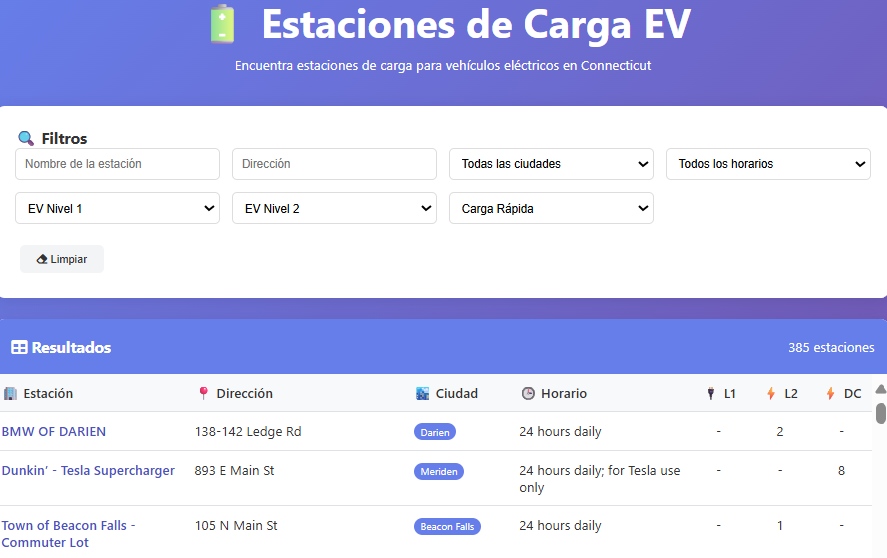
\includegraphics[width=0.8\textwidth]{Imagenes/presentacion1.png} % Cambia la ruta por la imagen real

  La aplicación muestra datos de estaciones con filtros avanzados y estilizado usando XSLT + CSS
  \end{center}
  \end{frame}

% FUNDAMENTOS DE XSLT
\section{Fundamentos de XSLT}

\begin{frame}
\frametitle{¿Qué veremos en esta sección?}
Explicaremos los conceptos básicos de XSLT y cómo se usa para transformar datos XML en páginas web.
\end{frame}

\begin{frame}[fragile]
\frametitle{¿Cómo funciona XSLT?}
\begin{itemize}
    \item Recibe datos en formato XML (en nuestro caso, de la API de estaciones de carga)
    \item Usa una hoja de estilo (archivo \texttt{estilos.xslt}) para definir cómo se verán esos datos
    \item El resultado es una página HTML lista para mostrar al usuario
    \item En nuestra aplicación, Flask maneja la obtención y transformación del XML
\end{itemize}
\begin{lstlisting}[language=Python]
# Como se procesa en app.py (version conceptual)
xml_data = obtener_xml_data()  # Obtiene XML de la API
xslt_doc = etree.parse('estilos.xslt')
transform = etree.XSLT(xslt_doc)
html_resultado = transform(xml_data)  # XML transformado en HTML
\end{lstlisting}
\end{frame}

\begin{frame}[fragile]
\frametitle{Estructura básica de nuestro archivo XSLT}
\begin{lstlisting}[language=XML]
<?xml version="1.0" encoding="UTF-8"?>
<xsl:stylesheet version="1.0" xmlns:xsl="http://www.w3.org/1999/XSL/Transform">
  <xsl:output method="html" indent="yes"/>
  <xsl:template match="/">
    <html>
      <head>
        <!-- Metadatos, estilos CSS y titulo -->
      </head>
      <body>
        <!-- Estructura HTML generada dinamicamente -->
      </body>
    </html>
  </xsl:template>
</xsl:stylesheet>
\end{lstlisting}
\end{frame}

\begin{frame}[fragile]
\frametitle{Características clave de nuestro XSLT}
Nuestro archivo \texttt{estilos.xslt} incluye:
\begin{itemize}
    \item CSS embebido para estilizar completamente la aplicación
    \item JavaScript para manejo de interacciones del usuario
    \item Transformación de datos XML a elementos HTML
    \item Plantillas para componentes de interfaz reutilizables
    \item Lógica condicional para manejar casos especiales
\end{itemize}
\begin{lstlisting}[language=XML]
<!-- Ejemplo de estilizado en estilos.xslt -->
<style>
  .station-name {
    font-weight: 600;
    color: #4c51bf;
    display: flex;
    align-items: center;
    gap: 8px;
  }
</style>
\end{lstlisting}
\end{frame}

% ARQUITECTURA DEL PROYECTO
\section{Arquitectura del Proyecto}

  \begin{frame}
  \frametitle{¿Qué veremos en esta sección?}
  Mostraremos cómo se conectan las diferentes partes del proyecto: la fuente de datos, el backend, la transformación XSLT y el frontend.
  \end{frame}

  \begin{frame}
  \frametitle{Componentes principales}
  \begin{itemize}
      \item \textbf{API Externa}: Proporciona los datos en XML.
      \item \textbf{Flask (Python)}: Recibe los datos y aplica la transformación XSLT.
      \item \textbf{XSLT}: Convierte los datos XML en HTML.
      \item \textbf{Navegador}: Muestra la página web al usuario.
  \end{itemize}
  \end{frame}

  \begin{frame}
  \frametitle{Diagrama de arquitectura}
  \begin{center}
  \begin{tikzpicture}[node distance=2cm]
      \node (xml) [rectangle, draw, fill=blue!20, minimum width=3cm, minimum height=1cm] {API Externa (XML)};
      \node (flask) [rectangle, draw, fill=orange!20, minimum width=3cm, minimum height=1cm, below=of xml] {Flask (Python)};
      \node (xslt) [rectangle, draw, fill=green!20, minimum width=3cm, minimum height=1cm, right=of flask] {Transformaci\'on XSLT};
      \node (html) [rectangle, draw, fill=red!20, minimum width=3cm, minimum height=1cm, below=of xslt] {HTML (Web)};
      \draw[->, thick] (xml) -- (flask);
      \draw[->, thick] (flask) -- (xslt);
      \draw[->, thick] (xslt) -- (html);
  \end{tikzpicture}
  \end{center}
  \end{frame}

  % ESPACIO PARA IMAGEN DE LA APP (otra vista)
  \begin{frame}
  \frametitle{Datos no formateados}
  \begin{center}
  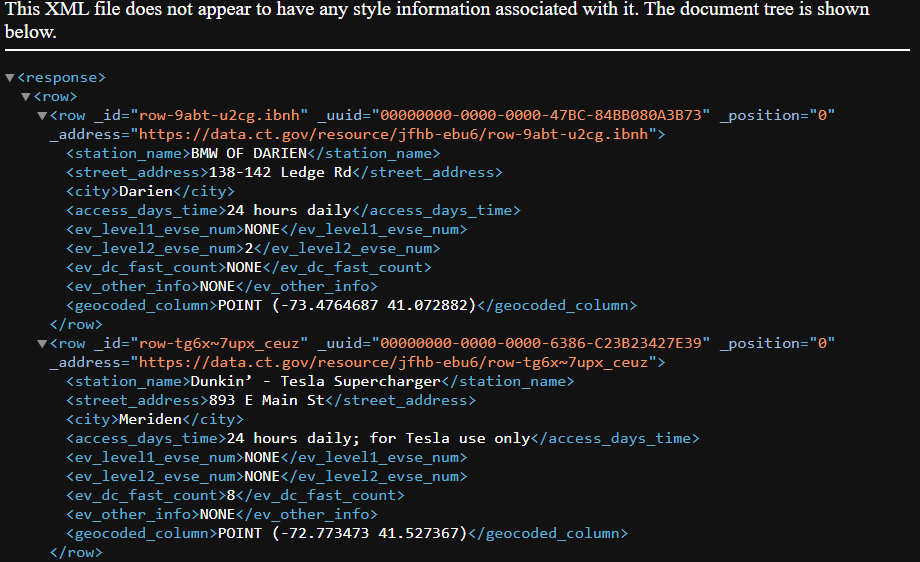
\includegraphics[width=0.8\textwidth]{Imagenes/Datos.png} % Cambia la ruta por la imagen real
  \end{center}
  \end{frame}

% FUNCIONAMIENTO DE XSLT EN EL PROYECTO
\section{Funcionamiento de XSLT en el Proyecto}

\begin{frame}
\frametitle{¿Qué veremos en esta sección?}
Veremos ejemplos concretos de cómo XSLT transforma los datos y cómo se integra con el backend en Python.
\end{frame}

\begin{frame}[fragile]
\frametitle{Ejemplo: Extracción de datos con XSLT}
\begin{lstlisting}[language=XML]
<td class="station-name">
  <xsl:value-of select="station_name"/>
</td>
\end{lstlisting}
Esto toma el nombre de la estación desde el XML y lo muestra en la tabla.
\end{frame}

\begin{frame}[fragile]
\frametitle{Ejemplo: Iteración sobre elementos}
\begin{lstlisting}[language=XML]
<xsl:for-each select="//row/row">
  <tr>
    <!-- Celdas de la tabla -->
  </tr>
</xsl:for-each>
\end{lstlisting}
Esto permite mostrar muchas estaciones, una por cada fila del XML.
\end{frame}

\begin{frame}[fragile]
\frametitle{Ejemplo: Lógica condicional}
\begin{lstlisting}[language=XML]
<xsl:choose>
  <xsl:when test="ev_level1_evse_num = 'NONE'">
    <span>Ninguno</span>
  </xsl:when>
  <xsl:otherwise>
    <xsl:value-of select="ev_level1_evse_num"/>
  </xsl:otherwise>
</xsl:choose>
\end{lstlisting}
Esto muestra "Ninguno" si no hay cargador de nivel 1, o el número si existe.
\end{frame}

% INTEGRACIÓN CON FLASK
\section{Integración con Flask}

\begin{frame}
\frametitle{¿Qué veremos en esta sección?}
Explicaremos cómo el backend en Python (Flask) obtiene los datos y aplica la transformación XSLT antes de mostrar la página al usuario.
\end{frame}

\begin{frame}[fragile]
\frametitle{Código clave en Flask}
  \begin{lstlisting}[language=Python]
@app.route('/')
def home():
    xml_data = obtener_xml_data()
    xslt_path = os.path.join(os.path.dirname(__file__), 'static', 'estilos.xslt')
    xslt_doc = etree.parse(xslt_path)
    transform = etree.XSLT(xslt_doc)
    resultado = transform(xml_data)
    return Response(str(resultado), mimetype='text/html')
  \end{lstlisting}
\end{frame}

% ESPACIO PARA IMAGEN DE LA APP (filtros)
\begin{frame}
\frametitle{Vista de los filtros en la aplicación}
\begin{center}
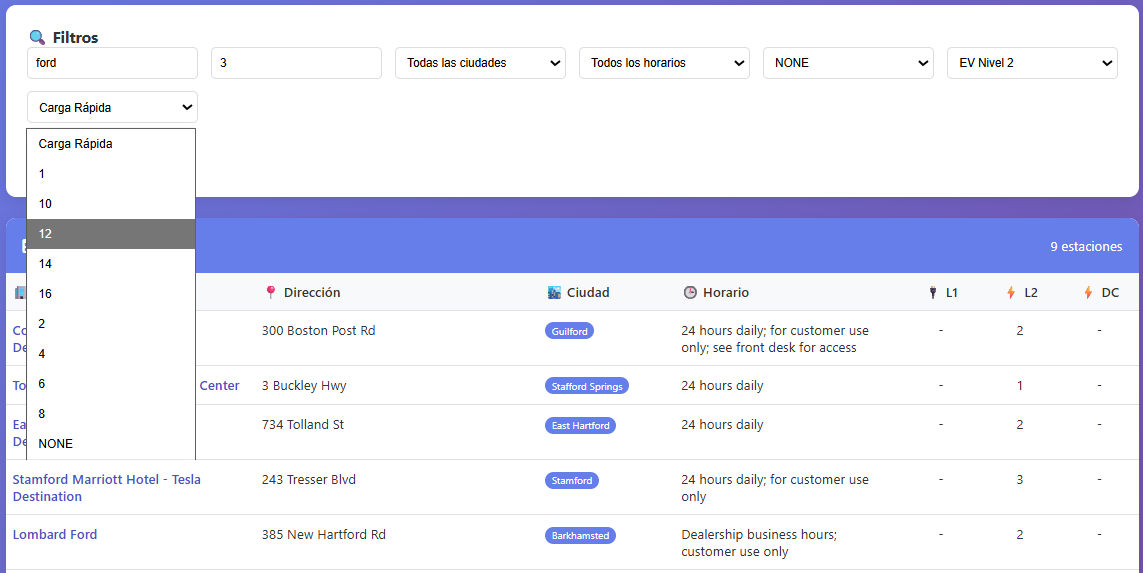
\includegraphics[width=0.8\textwidth]{Imagenes/filtros.png} % Cambia la ruta por la imagen real
\end{center}
\end{frame}

% VENTAJAS Y DESAFÍOS
\section{Ventajas y Desafíos}

%\begin{frame}
%\frametitle{¿Qué veremos en esta sección?}
%Comentaremos los puntos fuertes y los retos de usar XSLT en este tipo de proyectos.
%\end{frame}

\begin{frame}
\frametitle{Ventajas de usar XSLT}
\begin{itemize}
    \item Permite separar los datos de la presentación.
    \item Facilita el mantenimiento y la actualización de la interfaz.
    \item Es eficiente para transformar grandes volúmenes de datos XML.
    \item Permite generar HTML, CSS y JavaScript en un solo paso.
\end{itemize}
\end{frame}

\begin{frame}
\frametitle{Desafíos y limitaciones}
\begin{itemize}
    \item La sintaxis puede ser difícil para quienes no la conocen.
    \item Depurar errores en XSLT puede ser complicado.
    \item No es tan interactivo como frameworks modernos, pero se puede complementar con JavaScript.
\end{itemize}
\end{frame}

% POSIBLES MEJORAS
\section{Posibles Mejoras}

%\begin{frame}
%\frametitle{¿Qué veremos en esta sección?}
%Propondremos ideas para mejorar la aplicación en el futuro.
%\end{frame}

\begin{frame}
\frametitle{Ideas para el futuro}
\begin{itemize}
    \item Implementar caché para acelerar la carga.
    \item Añadir paginación para manejar más datos.
    \item Permitir exportar los datos filtrados.
    \item Mejorar la accesibilidad y el diseño visual.
    \item Integrar mapas interactivos.
\end{itemize}
\end{frame}

% CONCLUSIONES
\section{Conclusiones}

%\begin{frame}
%\frametitle{¿Qué veremos en esta sección?}
%Resumiremos los aprendizajes y la importancia de XSLT en el proyecto.
%\end{frame}

\begin{frame}
\frametitle{Conclusiones}
\begin{itemize}
    \item XSLT es una herramienta poderosa para transformar y mostrar datos XML.
    \item Su integración con Flask permite crear aplicaciones web modernas y eficientes.
    \item La separación entre datos y presentación facilita el mantenimiento.
    \item Aunque tiene retos, sigue siendo útil en muchos contextos.
\end{itemize}
\end{frame}

% PREGUNTAS
\begin{frame}
\frametitle{¿Preguntas?}
\begin{center}
\Huge ¡Gracias por su atención!
\end{center}
\end{frame}

\end{document} 